%------------------
% BULGULAR
%------------------
%\section{Sonuçlar} %Sonuçlar kısmında genellikle section olmaz gerekir ise
%\section{title} " %" kaldırılarak eklenir
% aşağıda mevcut örnek tablo ve figür komutlarından faydalanabilirsiniz
% % % % % % % % % % % % % % % % % % % % % % % % % % % % % % % % % % % % % % % % %
Toplam 293 hasta çalışmaya alınmıştı. Ortalama takip süresi 60 (30.0;102) aydı. Kohortun genel özellikleri Tablo \ref{tablo:kohortgenel}'de gösterilmiştir. 

 \begin{longtable}{lcc}\caption{Kohortun genel özellikleri}\label{tablo:kohortgenel}\\
    \hline
     &    N=293       &  N \\
     \hline
    Cinsiyet &                  & 293\\
$\qquad$Erkek &   151 (51.5\%)    &    \\
$\qquad$Kadın &   142 (48.5\%)    &    \\
Yaş &   47.3 (12.7)    & 293\\
Takip Süresi (Ay) & 60.0 [30.0;102]  & 293\\
Poliklinik Başvurusu & 18.0 [11.0;29.0] & 293 \\

    \hline
    \end{longtable}

Hastaların bakılan ilk ve son laboratuvar testlerinin sonuçları Tablo \ref{tablo:ilksonlab}'de gösterilmiştir. 6 hastada takip başlangıcında HBeAg pozitifti, takip sonunda ise hepsinde HBeAg serokonversiyonu oluşmuştu. Delta antikoru pozitif saptanmış hastalarda dış merkezde bakılan HDV RNA negatifti. 293 hastanın 18'i (\%6.2) HBsAg seroklirensi oluşmasına rağmen takip ediliyordu. Bu hastaların 6'sında (\%33) Anti-HBs oluşmuştu.   


    \begin{longtable}{lccc}\caption{Hastaların ilk ve en son yapılan testleri ve sonuçları} \label{tablo:ilksonlab}\\
    \hline
     &       ILK        &       SON        & \multirow{2}{*}{\textit{p}}\\
 &      N=293       &      N=293       &           \\

    \hline
    \hline
    \endfirsthead
    \multicolumn{4}{l}{\tablename\ \thetable{} \textit{-- önceki sayfadan devam ediyor}}\\
    \hline
     &       ILK        &       SON        & \multirow{2}{*}{p.overall}\\
 &      N=293       &      N=293       &           \\

    \hline
    \hline
    \endhead
    \hline
    \multicolumn{4}{l}{\textit{devam ediyor}} \\
    \endfoot
    \multicolumn{4}{l}{}  \\
    \endlastfoot
    ALT & 20.0 [16.0;28.0] & 20.0 [15.0;28.0] &   0.395  \\
    AST & 21.0 [17.0;24.0] & 19.0 [17.0;23.0] &   0.021  \\
    HBV DNA &  354 [107;1355]  &  236 [49.0;773]  &   0.001   \\
    HBeAg &                  &                  &   0.035  \\
    $\qquad$Pozitif &    6 (2.10\%)     &    0 (0.00\%)     &          \\
    $\qquad$Negatif &   280 (97.9\%)    &    232 (100\%)    &          \\
Anti-HBe &                  &                  &   0.005  \\
$\qquad$Pozitif &   277 (96.9\%)    &    228 (100\%)    &          \\
$\qquad$Negatif &    9 (3.15\%)     &    0 (0.00\%)     &          \\
Delta Antikoru &                  &                  &   0.637  \\
$\qquad$Pozitif &    3 (1.11\%)     &    1 (0.49\%)     &          \\
$\qquad$Negatif &   268 (98.9\%)    &   205 (99.5\%)    &          \\
HBsAg & & & \\
$\qquad$Pozitif &    293 (100\%)     &    275 (93.8\%)     &          \\
$\qquad$Negatif &    0 (0.00\%)    &   18 (6.2\%)    &          \\


    \hline
    \end{longtable}

 
Hastalara yapılan laboratuvar, görüntüleme ve biyopsi tetkiklerinin toplam sayısı ve toplam maliyet Tablo \ref{tablo:toplamsayi}'te gösterilmiştir. En çok istenmiş tetkik ALT idi. Toplam maliyeti en fazla olan test HBV DNA idi. KC biyopsisi toplam en az yapılmış 2. test olmasına rağmen HBV DNA'dan sonra toplam maliyette 2. sıradaydı.


\begin{longtable}{L{5.5cm}cc}\caption{Hastalara yapılan tetkiklerin toplam sayısı ve toplam maliyet} \label{tablo:toplamsayi}\\
    \hline
     Test & Toplam sayı & Toplam Maliyet (TL) \\ 

   
    \hline
    \endfirsthead
    \multicolumn{3}{l}{\tablename\ \thetable{} \textit{-- önceki sayfadan devam ediyor}}\\
    \hline
     Test & Toplam sayı & Toplam Maliyet (TL) \\ 
    \hline
   
    \endhead
    \hline
    \multicolumn{3}{l}{\textit{devam ediyor}} \\
    \endfoot
    \multicolumn{3}{l}{}  \\
    \endlastfoot
             Hemogram & 2421 & 7989 \\
             ALT & 3019 & 3653 \\
             AST & 2839 & 3123 \\
             Albumin & 1023 & 1125 \\
             PT-APTT-INR & 489 & 3227 \\
             AFP & 1783 & 12748 \\
             Anti HCV & 321 & 2825 \\
             Anti HIV & 186 & 1534 \\
             Anti HAV IgG & 200 & 1760 \\
             Anti HBc IgM & 20 & 176 \\
             Anti HBc IgG & 100 & 880 \\
             HBsAg & 1392 & 11484 \\
             Anti-HBs & 664 & 5843 \\
             HBeAg & 918 & 7574 \\
             Anti-HBe & 852 & 7498 \\
             HBV DNA & 2401 & 268599.87 \\
             Delta Antikoru & 675 & 6311 \\
             Hepatobilier USG & 115 & 1290 \\
             Üst batın USG & 736 & 12387 \\
             Tüm batın USG & 358 & 9372 \\
             Üst batın MR & 63 & 6757 \\
             KC biyopsisi & 43 & 12900 \\
             
                 \hline
                 \end{longtable}


37 hastaya toplam 43 KC biyopsisi yapılmıştı. 37 hastanın biyopsi anında ALT ve HBV DNA değerleri Tablo \ref{tablo:biyopsi}'te gösterilmiştir. En çok biyopsi kararı ALT normal düzeyde, HBV DNA ise 2000 ile 20000 IU/ml arasında olan hastalara verilmiştir.

\bigskip

%\begin{\begin{landscape}
\begin{minipage}[c]{\textwidth}
\renewcommand{\arraystretch}{1} %SATIR ARALI^GI BEL'IRLEMEK 'IÇ'IN SAYIYI DE^G'I¸ST'IR'IN
\centering
\begin{threeparttable}
\caption{Biyopsi anındaki HBV DNA ve ALT düzeylerine göre hasta sayısı} \label{tablo:biyopsi} %Tablo ba¸slı^gı ve referans etiketi
%---------------------------------------
\begin{tabular}{lcc}
\hline
                          & ALT N (IU/L) & ALT yüksek (IU/L) \\
                          \hline
HBV DNA \textless2000 (IU/ml)     & 2     & 2          \\
HBV DNA 2000-20000  (IU/ml)       & 26    & 2          \\
HBV DNA \textgreater20000  (IU/ml) & 0     & 5 \\
\hline        
\end{tabular}
%------------------------------------------
\begin{tablenotes}
\footnotesize
\item İki defa biyopsi yapılmış hastalarda son biyopsi dikkate alınmıştır.
\end{tablenotes}
\end{threeparttable}
\end{minipage}
%\end{landscape}}

\bigskip

ALT normal iken biyopsi yapılmış 28 hastanın 10'unun fibroz skoru 0, 17'sinin 1, 1'inin ise 2 idi. ALT yüksek iken biyopsi yapılmış 9 hastanın 4'ünün fibroz skoru 0, 5'inin ise 1 idi.






                

Testlerin kişi başına toplam maliyeti ise Tablo \ref{tablo:toplamveyuzde}'te gösterilmiştir. Kişi başı tetkik masrafının \%69'unu HBV DNA oluşturmaktadır. 

\begin{longtable}{L{5.5cm}cc}\caption{Kişi başına toplam harcama ve yüzdeleri} \label{tablo:toplamveyuzde}\\
    \hline
     Test & Toplam TL/kişi & \% Toplam \\ 

   
    \hline
    \endfirsthead
    \multicolumn{3}{l}{\tablename\ \thetable{} \textit{-- önceki sayfadan devam ediyor}}\\
    \hline
     Test & Toplam TL/kişi & \% Toplam \\ 
    \hline
   
    \endhead
    \hline
    \multicolumn{3}{l}{\textit{devam ediyor}} \\
    \endfoot
    \multicolumn{3}{l}{}  \\
    \endlastfoot
	Hemogram & 27,27 &	2,05\% \\
	ALT & 12,47 &	0,94\% \\
	AST & 10,66 &	0,80\% \\
	Albumin & 3,84 &	0,29\% \\
	PT-APTT-INR & 11,01&	0,83\% \\
	AFP & 43,51&	3,28\% \\
	Anti-HCV & 9,64 &	0,73\% \\
	Anti-HIV & 5,24 &	0,39\% \\
	Anti-HAV IgG & 6,01 &	0,45\% \\
	Anti-HBc IgM & 0,60 &	0,05\% \\
	Anti-HBc IgG & 3,00 &	0,23\% \\
	HBsAg & 39,19 &	2,95\% \\
	Anti-HBs & 19,94 &	1,50\% \\
	HBeAg & 25,85 &	1,95\% \\
	Anti-HBe & 25,59 &	1,93\% \\
	HBV DNA & 916,72 &	69,04\% \\
	Delta Antikoru & 21,54 &	1,62\% \\
	Hepatobilier USG & 4,40 &	0,33\% \\
	Üst batın USG & 42,28 &	3,18\% \\
	Tüm batın USG & 31,99 &	2,41\% \\
	Üst batın MR & 23,06 &	1,74\% \\
	KC biyopsisi & 44,03 &	3,32\% \\
\hline
                 \end{longtable}

Hastalar takip süresine göre kategorize edildiğinde 0-36 ay arasında takip edilmiş hastalarda vizit başına toplam maliyet en fazlaydı. Masrafın çoğunu HBV DNA oluşturuyordu (Tablo \ref{tablo:tlvizit}). 


  \begin{longtable}{lcccc}\caption{Takip süresine göre testlerin vizit başına maliyeti} \label{tablo:tlvizit}\\
      \hline
        & 0-36 Ay & 36-72 Ay & 72-108 Ay & 108-150 Ay \\ 
  
     
      \hline
      \endfirsthead
      \multicolumn{5}{l}{\tablename\ \thetable{} \textit{-- önceki sayfadan devam ediyor}}\\
      \hline
        & 0-36 & 36-72 & 72-108 & 108-150 \\ 
      \hline
     
      \endhead
      \hline
      \multicolumn{5}{l}{\textit{devam ediyor}} \\
      \endfoot
      \multicolumn{3}{l}{}  \\
      \endlastfoot
   Hemogram & 1.32 & 1.29 & 1.25 & 1.29 \\ 
   ALT & 0.54 & 0.53 & 0.63 & 0.60 \\ 
   AST & 0.48 & 0.45 & 0.54 & 0.51 \\ 
   Albumin & 0.23 & 0.19 & 0.17 & 0.18 \\ 
   PT-APTT-INR & 0.60 & 0.43 & 0.58 & 0.47 \\
   AFP & 2.47 & 2.23 & 1.98 & 1.95 \\ 
   Anti-HCV & 0.76 & 0.40 & 0.48 & 0.43 \\ 
   Anti-HIV & 0.44 & 0.24 & 0.24 & 0.25 \\ 
   Anti-HAV IgG & 0.69 & 0.45 & 0.14 & 0.27 \\  
   Anti-HBc IgM & 0.03 & 0.05 & 0.02 & 0.02 \\ 
   Anti-HBc IgG & 0.34 & 0.17 & 0.11 & 0.11 \\ 
   HBsAg & 2.46 & 2.22 & 1.60 & 2.02 \\ 
   Anti-HBs & 1.15 & 1.05 & 0.92 & 0.92 \\ 
   HBeAg & 1.99 & 1.28 & 1.05 & 1.34 \\ 
   Anti-HBe & 2.08 & 1.31 & 0.96 & 1.37 \\ 
   HBV DNA & 54.12 & 49.40 & 37.74 & 44.01 \\ 
   Delta Antikoru & 1.84 & 1.27 & 0.72 & 0.96 \\ 
   Hepatobilier USG & 0.29 & 0.22 & 0.16 & 0.18 \\ 
   Tüm Batın USG & 2.58 & 2.49 & 0.96 & 1.37 \\ 
   Üst Batın USG & 2.17 & 2.14 & 1.91 & 2.10 \\ 
   Üst Batın MR & 0.89 & 1.57 & 0.59 & 1.35 \\ 
   KC Biyopsisi & 1.85 & 1.79 & 1.17 & 2.05 \\
   \hline
   TOPLAM (TL) & 79.32 & 71.17 & 54.05 & 63.75 \\
  \hline
                   \end{longtable}
                   


Vizit başı toplam masraf, takip süresi arttıkça 36-72 ay ve 72-108 ay takipli hastalarda düşerken, 108-150 ay takip edilmiş hastalarda yeniden artmaktaydı. Takip süresine göre ilk 3 senedeki bu kümelenme Şekil \ref{fig:Fig1} ve \ref{fig:Fig2}'de gösterilmiştir.  
   
  
\begin{minipage}{0.49\textwidth}
 \begin{center}
 	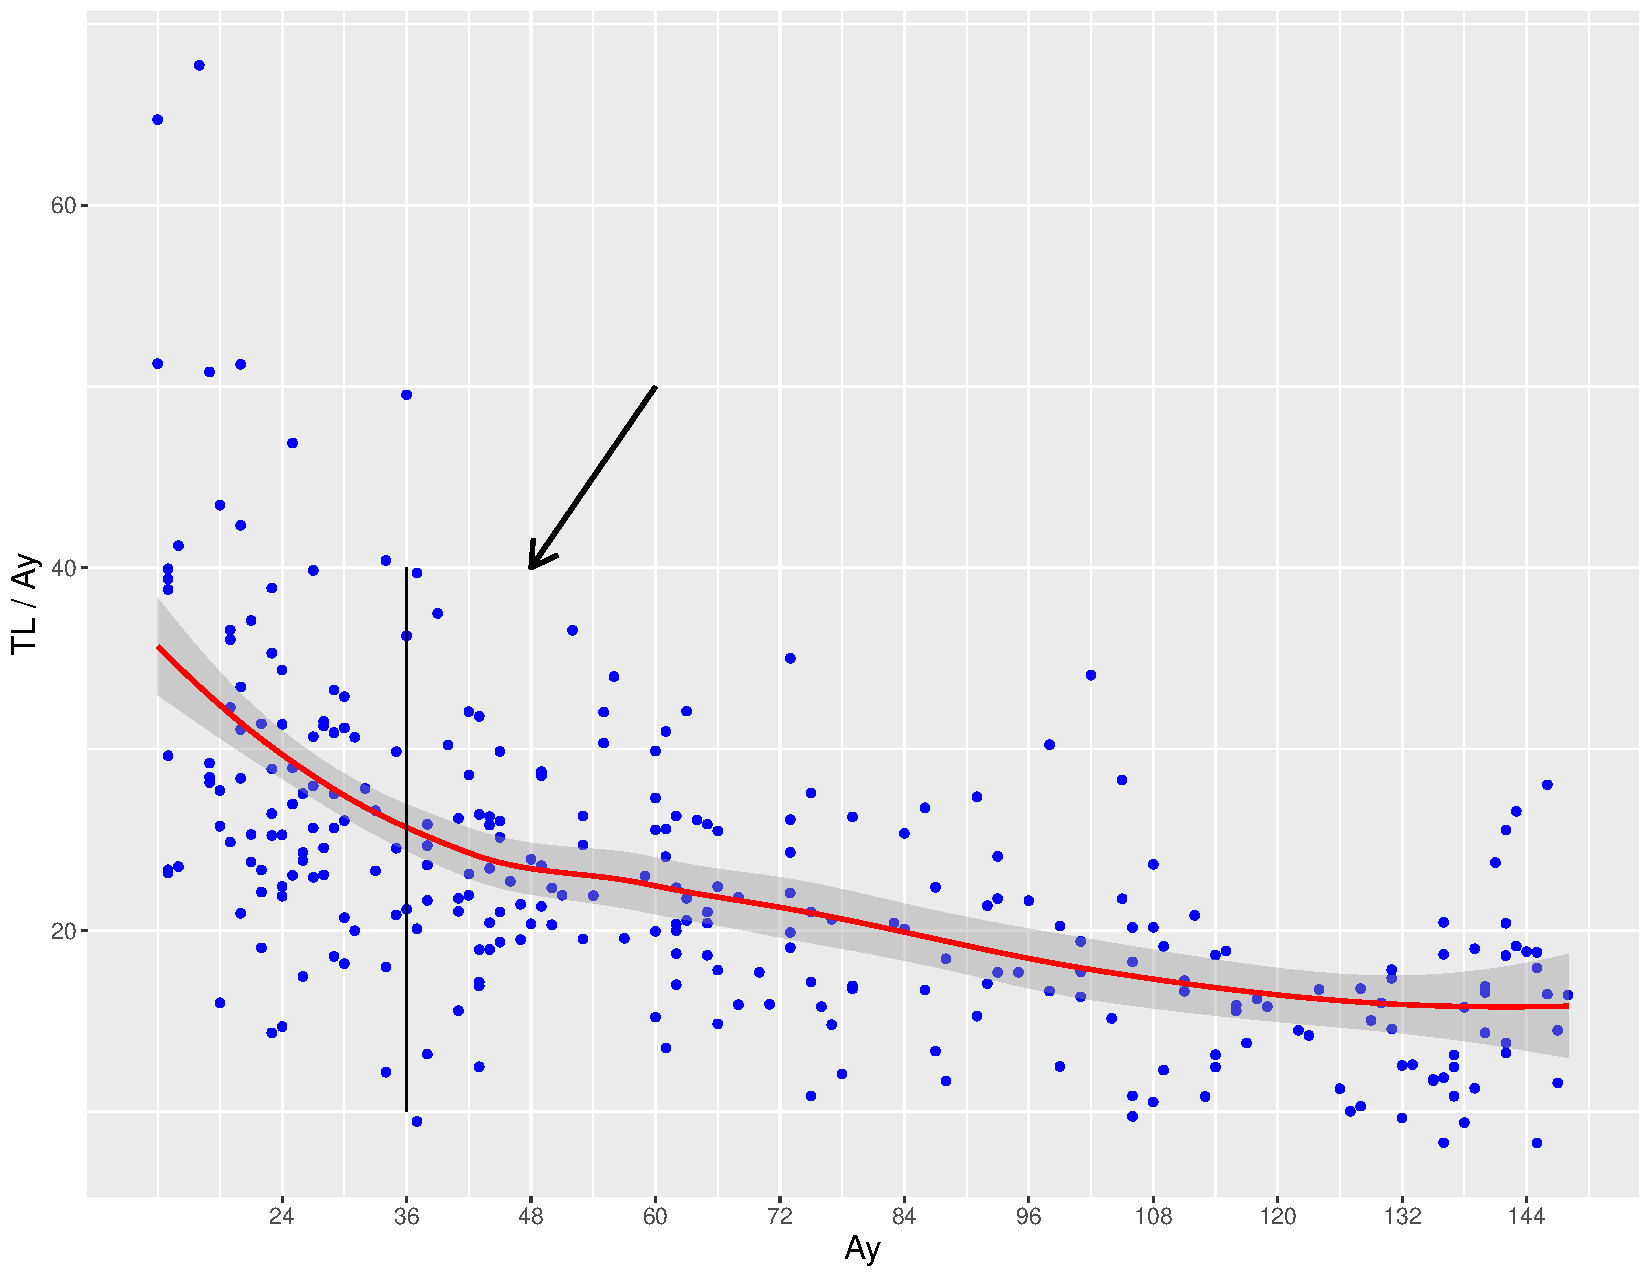
\includegraphics[width=1\linewidth, height=0.3\textheight]{../Figures/Fig1}
 	\end{center}
 	  %\vspace{0pt}
 	  \captionof{figure}{Aylara göre masraf kümelenmesi (TL/Ay)}
 	  \label{fig:Fig1}	
\end{minipage}
\begin{minipage}{0.49\textwidth}
	\begin{center}
	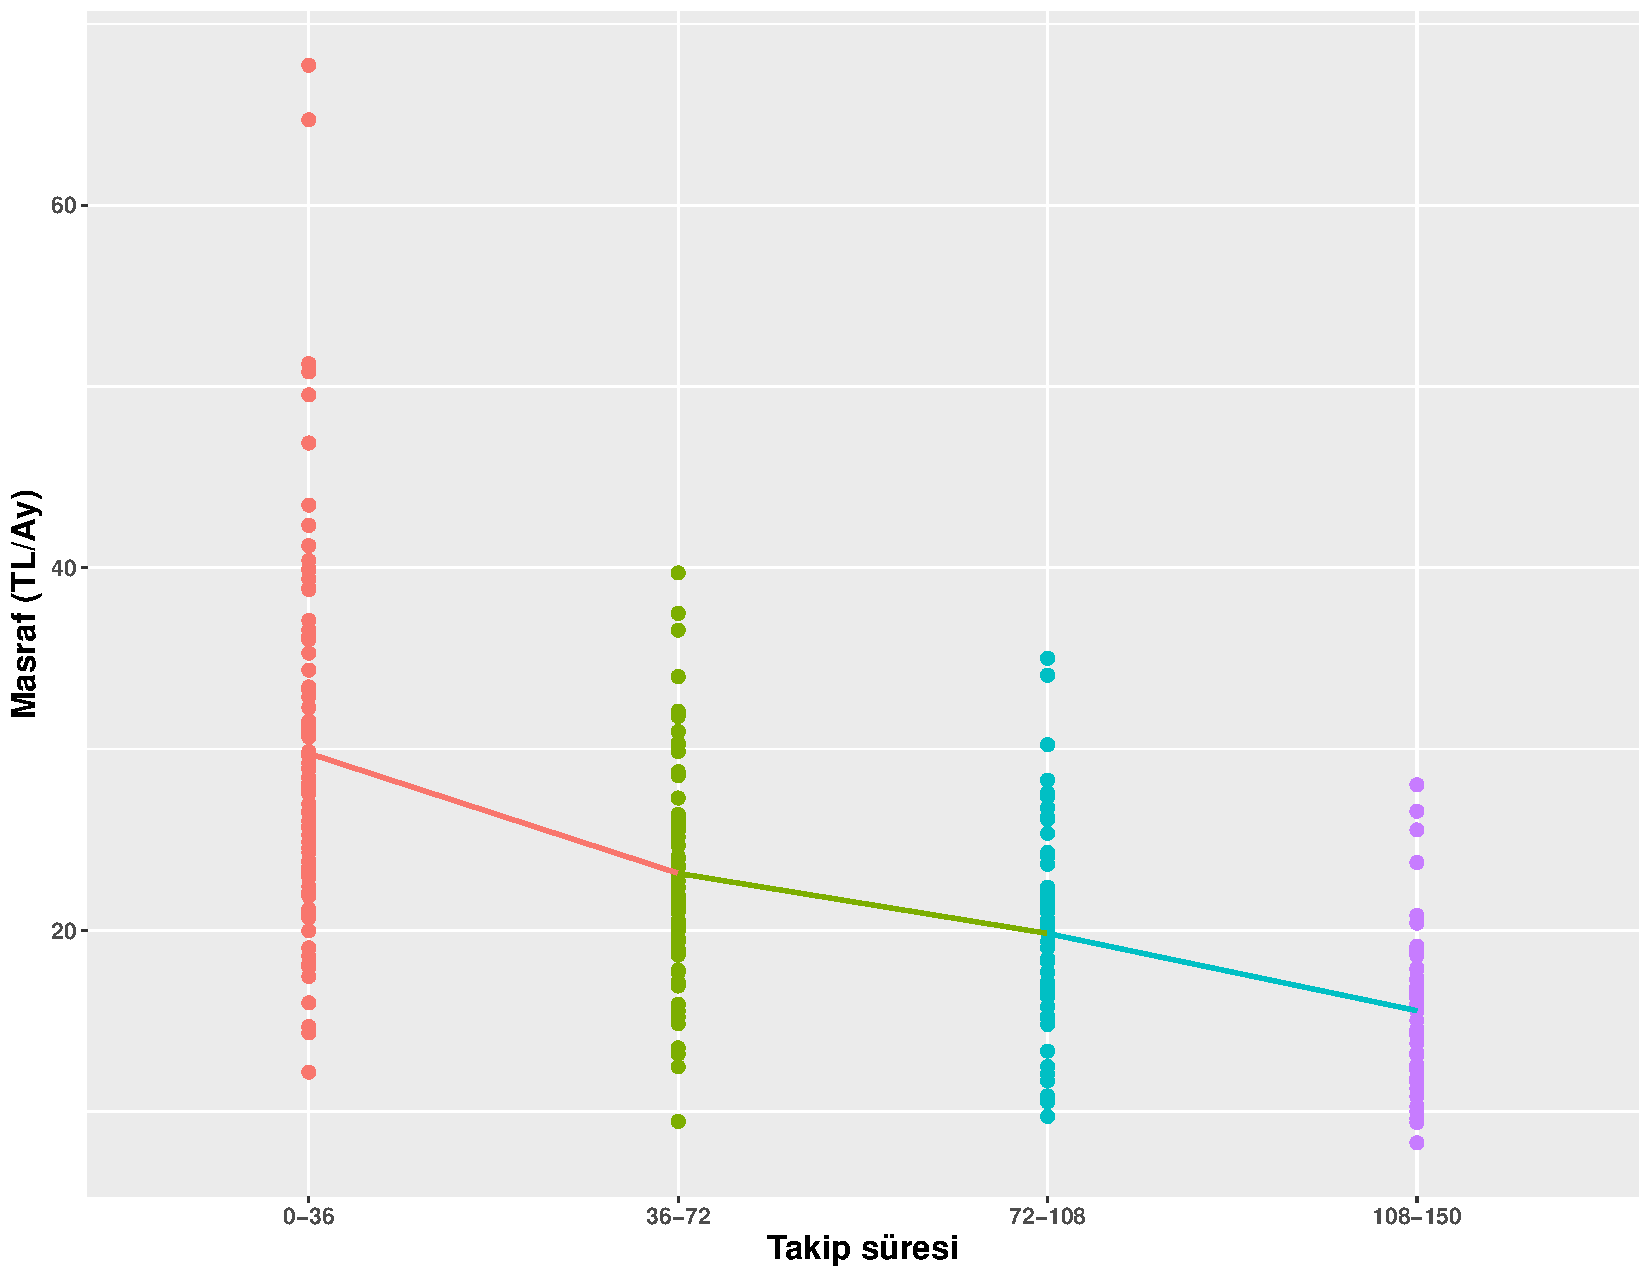
\includegraphics[width=1\linewidth, height=0.3\textheight]{../Figures/Fig2}
	\end{center}
	  %\vspace{0pt}
	  \captionof{figure}{Takip sürelerine göre masraf (TL/Ay)}
	  \label{fig:Fig2}
\end{minipage}\\  
  
  
  
Takip süresine göre testlerin hasta başına maliyeti Tablo \ref{tablo:tlhasta}'de gösterilmiştir. Oran olarak en çok masrafı HBV DNA oluşturmaktadır (Şekil \ref{fig:Fig5}). HBV DNA çıkartıldığında sırasıyla KC biyopsisi, AFP, üst batın USG ve HBsAg masrafı üstlenmektedir (Şekil \ref{fig:Fig6}) 
   
  
  \begin{longtable}{lcccc}\caption{Takip süresine göre testlerin hasta başına maliyeti} \label{tablo:tlhasta}\\
        \hline
          & 0-36 Ay & 36-72 Ay & 72-108 Ay & 108-150 Ay \\ 
    
       
        \hline
        \endfirsthead
        \multicolumn{5}{l}{\tablename\ \thetable{} \textit{-- önceki sayfadan devam ediyor}}\\
        \hline
          & 0-36 & 36-72 & 72-108 & 108-150 \\ 
        \hline
       
        \endhead
        \hline
        \multicolumn{5}{l}{\textit{devam ediyor}} \\
        \endfoot
        \multicolumn{3}{l}{}  \\
        \endlastfoot
  Hemogram & 12.03 & 22.34 & 47.93 & 36.67 \\ 
  ALT & 4.89 & 9.07 & 24.24 & 16.92 \\ 
  AST & 4.34 & 7.69 & 20.69 & 14.34 \\ 
  Albumin & 2.02 & 3.12 & 6.58 & 4.86 \\ 
  PT-APTT-INR & 5.35 & 6.68 & 23.15 & 13.32 \\
  AFP & 21.45 & 36.65 & 75.59 & 54.10 \\
  Anti-HCV & 5.96 & 6.17 & 18.30 & 11.29 \\ 
  Anti-HIV & 3.39 & 3.51 & 8.90 & 6.85 \\ 
  Anti-HAV IgG & 5.57 & 6.37 & 5.31 & 6.97 \\
  Anti-HBc IgM & 0.29 & 0.71 & 0.70 & 0.83 \\ 
  Anti-HBc IgG & 2.64 & 2.83 & 3.91 & 2.82 \\   
  HBsAg & 20.72 & 36.41 & 57.75 & 53.08 \\ 
  Anti-HBs & 9.88 & 17.40 & 33.66 & 24.91 \\ 
  HBeAg & 16.68 & 21.24 & 36.93 & 35.80 \\ 
  Anti-HBe & 17.21 & 21.34 & 34.22 & 36.53 \\ 
  HBV DNA & 469.85 & 828.10 & 1433.00 & 1207.35 \\ 
  Delta Antikoru & 14.75 & 20.74 & 27.90 & 26.82 \\ 
  Hepatobilier USG & 2.99 & 3.74 & 6.59 & 5.29 \\ 
  Tüm Batın USG & 20.36 & 39.72 & 34.91 & 35.57 \\ 
  Üst Batın USG & 18.70 & 36.56 & 69.72 & 59.06 \\ 
  Üst Batın MR & 8.34 & 28.35 & 25.54 & 36.42 \\ 
  KC biyopsisi & 23.33 & 34.48 & 57.14 & 79.25 \\
   \hline
                      \end{longtable}




\begin{minipage}{0.49\textwidth}
 \begin{center}
 	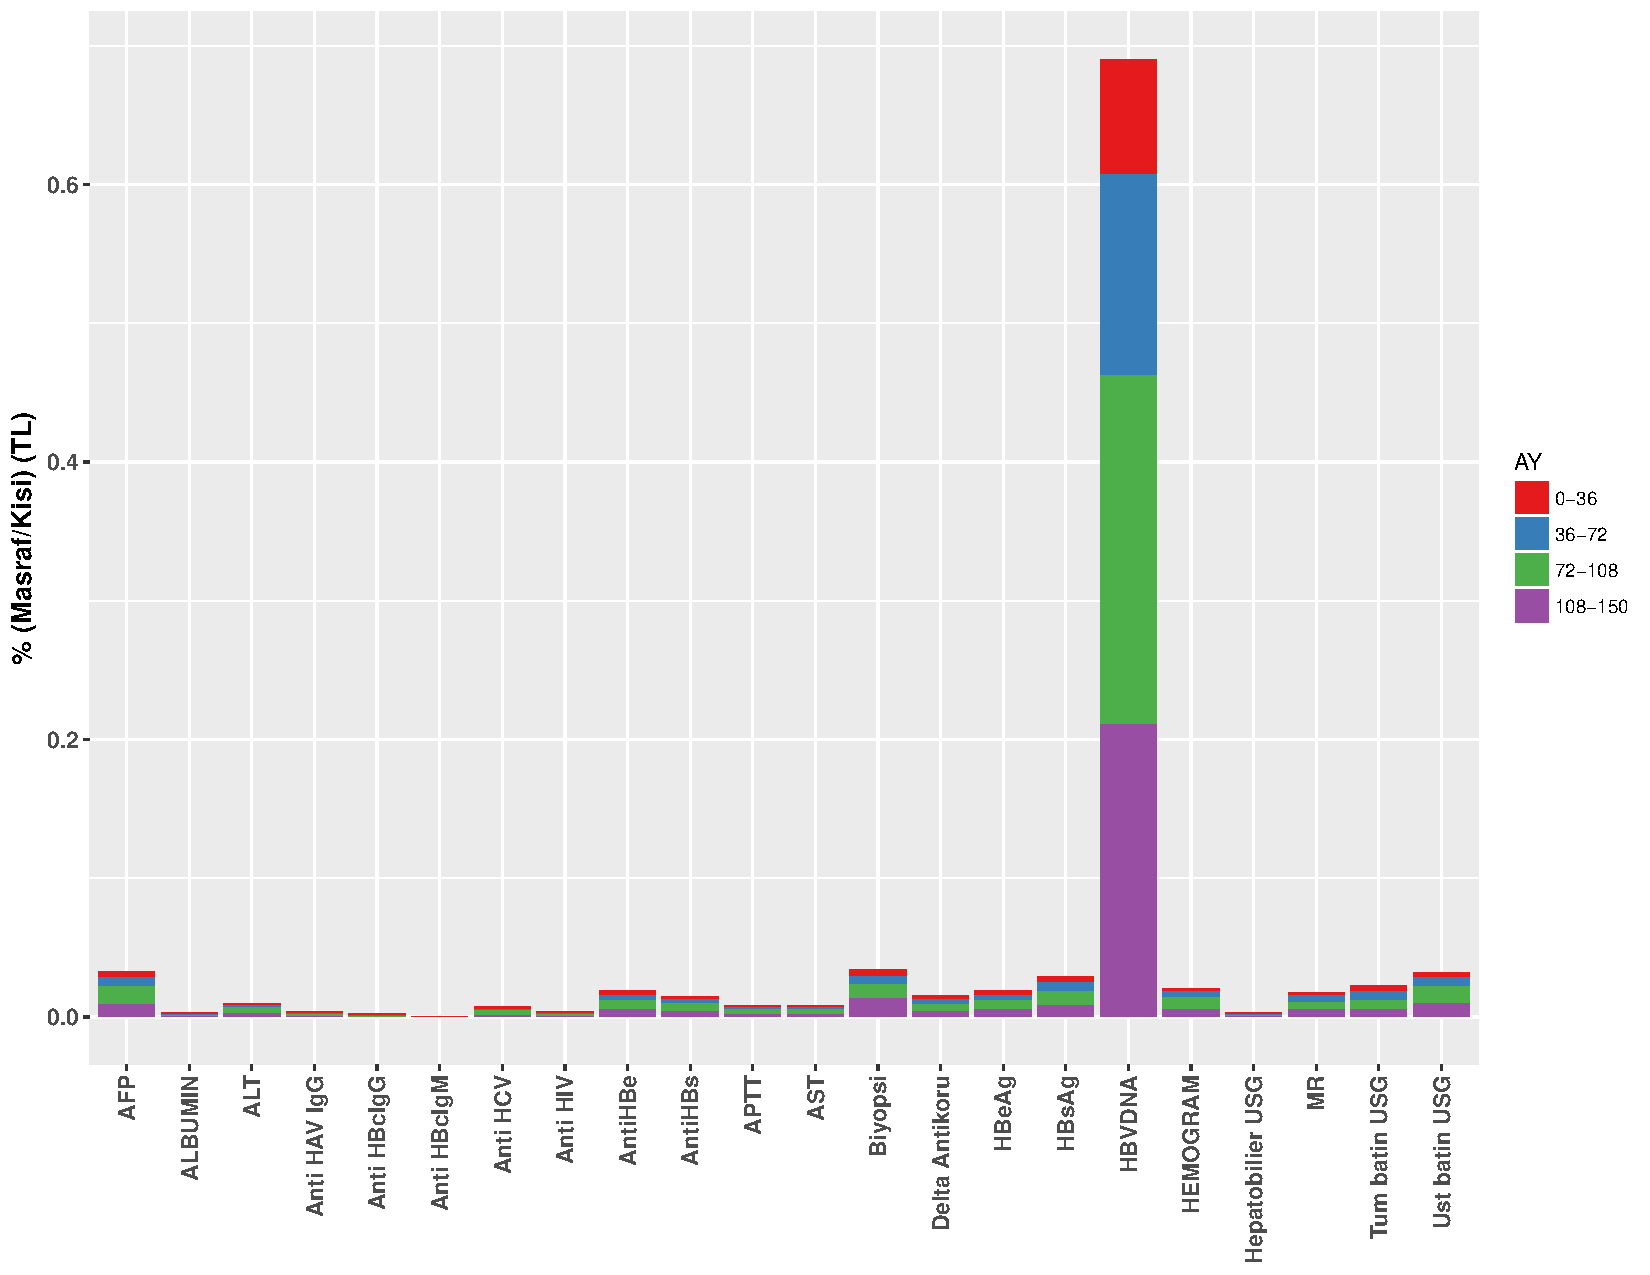
\includegraphics[width=1\linewidth, height=0.35\textheight]{../Figures/Fig5}
 	\end{center}
 	  %\vspace{0pt}
 	  \captionof{figure}{Takip süresine göre hasta başı maliyette testlerin yüzdeleri}
 	  \label{fig:Fig5}	
\end{minipage}
\begin{minipage}{0.49\textwidth}
	\begin{center}
	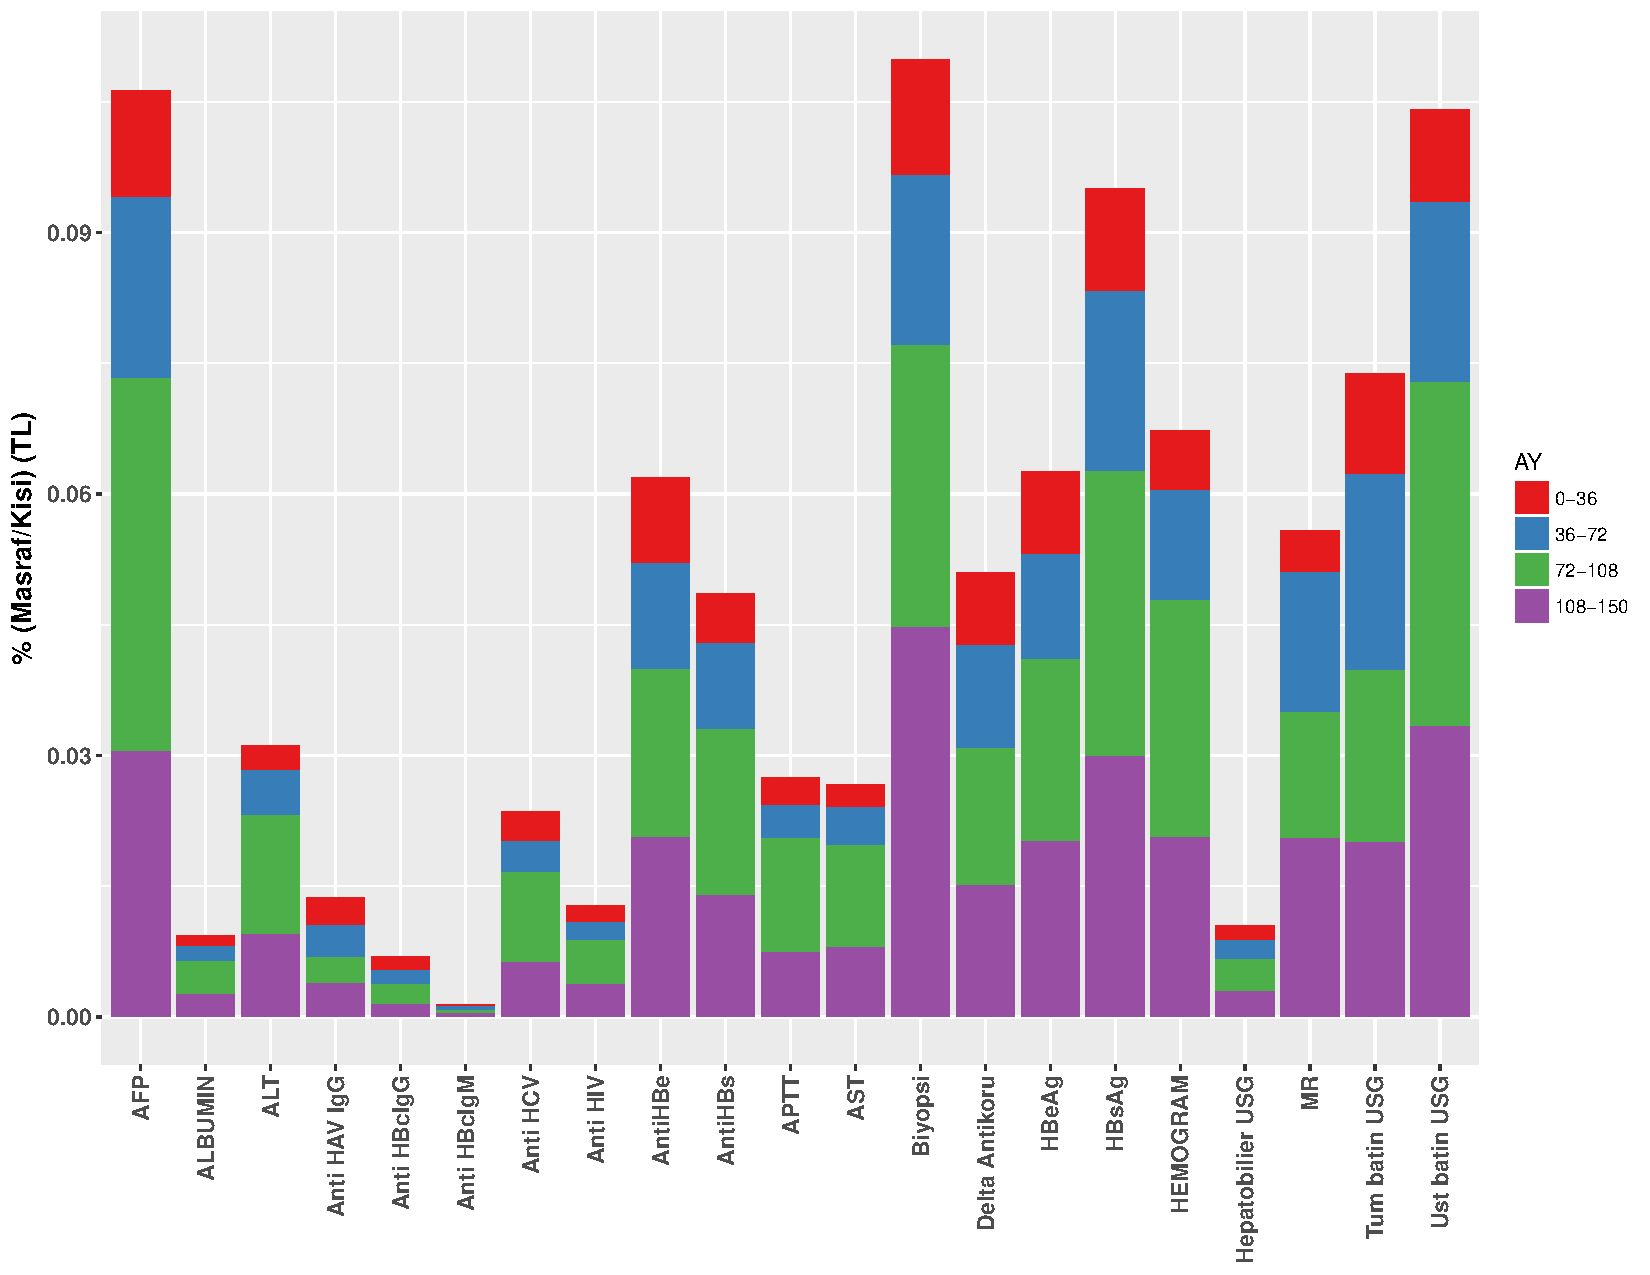
\includegraphics[width=1\linewidth, height=0.35\textheight]{../Figures/Fig6}
	\end{center}
	  %\vspace{0pt}
	  \captionof{figure}{Takip süresine göre hasta başı maliyette HBV DNA çıkartıldığında testlerin yüzdeleri}
	  \label{fig:Fig6}
\end{minipage}\\  









